\section{Bilderkennung- detection}

\subsection{Anfertigung der Bilder entlang der Strassen}
Damit das Convnet die Einteilung zwischen Zebrastreifen und Nicht-Zebrastreifen machen kann, braucht es ein RBG Bild mit 50 x 50 Pixeln als Input. Diese Inputbilder werden aus dem gedownloadetem Orthofoto ausgeschnitten. Mithilfe der Strassenkoordinaten muss nicht das ganze Orthofoto in kleine Bilder aufgeteilt, sondern die Inputbilder können nur entlang der Strassen ausgeschnitten werden. Der Abstand zwischen zwei Inputbildern (auch Schrittweite) ist so gewählt, das eine gewisse Überlappung vorliegt.
\\
\decision{Eckdaten Anfertigung Inputbilder} 
Die Inputbilder für das Convnet sind 50 x 50 Pixel gross, da auf Zoomstufe 19 50 Pixel etwa der Breite von zwei Strassen entspricht. Die Schrittweite wurde so angepasst, dass auch Zebrastreifen, die zwischen zwei Inputbildern liegen, erkannt werden.
\\
\begin{figure}[H]
	\centering
	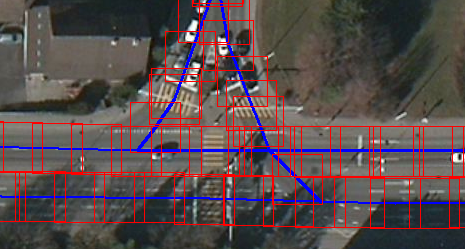
\includegraphics{images/squared_images.png}
	\caption{Blau: Strassenverlauf, Rot: Ausgeschnittene Bilder 50 x 50 Pixel. Diese Visualisierung der Inputbilder kann für jede beliebige BBox selbst durchgeführt werden. Siehe dazu examples/VisualizeSquaredImages.py im Projektordner}
\end{figure}



\subsection{Convnet}
Wir verwenden ein Convolutional Neuronal Network (Convnet) um die automatische Einteilung von Zebrastreifen und Nicht-Zebrastreifen zu machen. Um ein Convnet verwenden zu können, muss man es zuerst mit entsprechendem Bildmaterial trainieren. Wir sprechen hier Inputbilder, welche zum Teil automatisch mithilfe der Open Street Map Datenbank generiert werden konnten, aber meistens von Hand erstellt werden mussten. Wir haben uns während dieses Projektes ein Datenset aus über 4'400 Zebrastreifen- und 32'000 Nicht-Zebrastreifenbilder erarbeitet, um dies zu bewerkstelligen. Diese Arbeit beinhaltete stundelanges Aussortieren von Bildern.
\\

\begin{figure}[H]
	\centering
	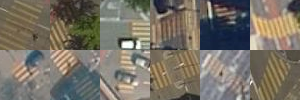
\includegraphics{images/Zebrastreifen_examples.png}
	\caption{6 x 2 Beispiele für Zebrastreifen. Wie auf den Bildern zu sehen ist, verdecken immer wieder Gegenstände das gelbe Muster. Die unterschiedliche Bildqualität der Orthofotos behinderte das Erkennen stark.}
\end{figure}

\begin{figure}[H]
	\centering
	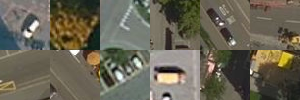
\includegraphics{images/No_Zebrastreifen_examples.png}
	\caption{6 x 2 Beispiele für Nicht-Zebrastreifen. Das Nicht-Zebrastreifen Set beinhaltet alle möglichen Strassensituationen von Stadt bis Land. Besonders bei gelben Autos oder Strassenmarkierungen hat das Convnet mühe.}
\end{figure}
